This assignment is about 2-dimensional vectors. A 2-dimensional vector or just a vector is a geometric object consisting of a direction and a length. Typically, vectors are represented as a coordinate pair $\vec v  = (x, y)$. The vector's ends are called its tail and tip, and when the tail is placed in $(0, 0)$, then its tip will be in the  $(x, y)$. Vectors have a number of standard operations on them:
\begin{align}
  \vec v_1 &= (x_1, y_1)
  \\\vec v_2 &= (x_2, y_2)
  \\\vec v_1 + \vec v_2 &= (x_1+x_2, y_1+y_2) \label{eq:addition}
  \\a \vec v_1 &= (a x_1, a y_1)  \label{eq:scalarMul}
\end{align}
Addition can be drawn as shown in \Cref{fig:vectorAddition}.
\begin{figure}
  \centering
  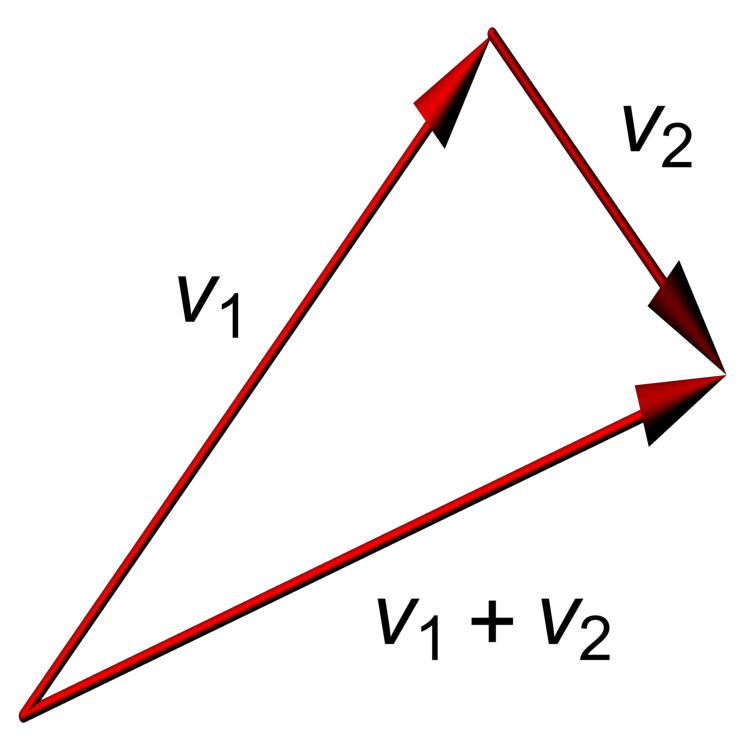
\includegraphics[width=0.28\textwidth]{vectorAddition}
  \caption{Illustration of vector addition in two dimensions.}
  \label{fig:vectorAddition}
\end{figure}
Rotation of a vector counter-clockwise around its tail by $a$ can be done as,
\begin{equation}
  R_a \vec v_1 = (x\cos(a) - y\sin(a),x\sin(a)+y\cos(a)) \label{eq:rotation}
\end{equation}
In F\#, the trigonometric functions are found in \lstinline{cos} and \lstinline{sin}, and they both take an angle in radians as the argument. The constant $\pi$ is found in \lstinline{System.Math.PI}. In the following, we will use the type abbreviation:
\begin{quote}
  \mbox{\lstinline!type vec = float * float!}
\end{quote}
